\documentclass[12pt,a4paper]{article}					% general format	


%%%% Charset
\usepackage[utf8]{inputenc}
\usepackage[russian]{babel}


%%%% Math
\usepackage{amsmath}
\usepackage{amsfonts}
\usepackage{amssymb}


%%%% Graphics
\usepackage{graphics}
\usepackage[pdftex]{graphicx}
\usepackage{lscape}
\usepackage{listings}
\usepackage[left=2.5cm, right=3cm, top=2cm, bottom=20mm]{geometry}

\renewcommand{\baselinestretch}{1.5}
\pagestyle{plain}
\usepackage{placeins}



\begin{document}
\thispagestyle{empty}
\begin{center}
\large Санкт-Петербургский политехнический университет\\
Институт компьютерных наук и технологий\\
Кафедра компьютерных систем и программных технологий\\
\vspace{55mm}
\Large Доклад по дисциплине "Распознавание образов"\\
\LARGE\textbf{Мультибиометрическое распознавание \\ с использованием изображений лица и уха}
\end{center}

\vspace{40mm}
\begin{flushright}
\large Выполнил: студент группы 53501/3\\ Дедков С. В.\\ Преподаватель: Никитин К. В.
\end{flushright}
\vspace{40mm}

\begin{center}
Санкт-Петербург\\ 2015
\end{center}

\newpage
\tableofcontents
\newpage

%------------------------------------------------

\section{Цель работы}

В данной работе рассматриваются техники мультибиометрического распознавания с использованием изображений ушей и лица.


%------------------------------------------------

\section{Введение}

\begin{itemize}

\item[-] Место: часть тела, которую необходимо распознать (например, ухо)
\item[-] Сенсор: механизм для получения биометрической информации (например, камера)
\item[-] Алгоритм: процедура сопоставления между биометрическими сигнатурами
\item[-] Режим: комбинация места, сенсора и алгоритма
\item[-] Мульти-экземпляр: использование нескольких наборов данных полученных используя какое-либо место, сенсор и режим
\item[-] Мульти-сенсор: использование нескольких сенсоров(и возможно, алгоритмов) для захвата данных какого-либо места
\item[-] Мульти-алгоритм: использование нескольких алгоритмов сопоставления на одних и тех же данных

\end{itemize}

Мультибиометрия подразумевает слияние данных на одном из уровне распознавания.
Способ комбинации будет влиять на качество распознавания системы.

Для определения уровней комбинирования в мультибиометрических системах ниже приведен элементарный биометрический процесс, а также блоки, входящие в него, на примере системы аутентификации. 
На рисунке 1 показана блок-схема элементарного биометрического процесса.

\begin{figure}[h!]
\centering
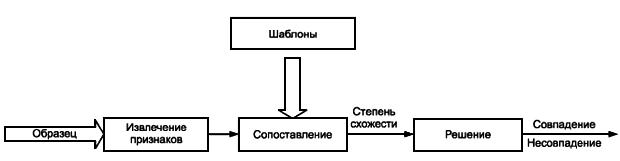
\includegraphics[scale=0.60]{res/bio_process}
\caption{Элементарный (универсальный) биометрический процесс}
\end{figure}

Биометрический образец, полученный с биометрического датчика (например, изображение отпечатка пальца), направляется в модуль извлечения признаков. В модуле извлечения признаков с помощью методов обработки сигналов происходит преобразование образца в признаки (например, контрольные точки отпечатка пальца), формирующее представление, подходящее для процесса сопоставления. Как правило, несколько признаков собираются в вектор признаков. На вход модуля сопоставления поступает вектор признаков, который сравнивается с имеющимся шаблоном. Результатом является степень схожести, которая используется в модуле принятия решения для определения (например, с помощью порога), соответствует ли представленный образец имеющемуся шаблону. Результат данного решения является бинарным: соответствует или не соответствует.

В мультибиометрии выделяют несколько уровней, на которых может происходить объединение:
\begin{itemize}
\item уровень принятия решения: каждый элементарный биометрический процесс на выходе предоставляет булев результат; эти результаты объединяются с помощью комбинирующего алгоритма, такого как логические функции "И" и "ИЛИ", используя параметры, такие как показатели качества образца, в качестве входных данных;

\begin{figure}[h!]
\centering
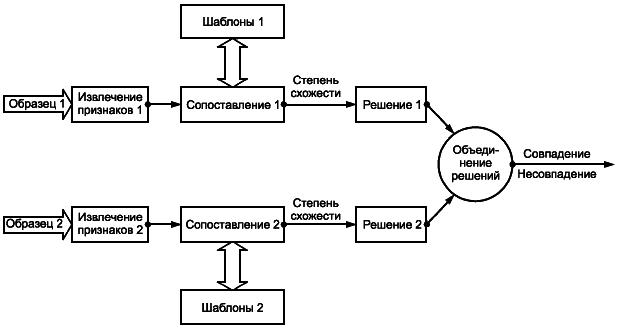
\includegraphics[scale=0.60]{res/bio_a}
\caption{объединение на уровне принятия решения}
\end{figure}

\item уровень степеней схожести: каждый элементарный биометрический процесс, как правило, предоставляет на выходе одну или несколько степеней схожести, которые объединяются в одну степень схожести или одно решение, в дальнейшем сопоставляемое с порогом принятия решения системы;

\begin{figure}[h!]
\centering
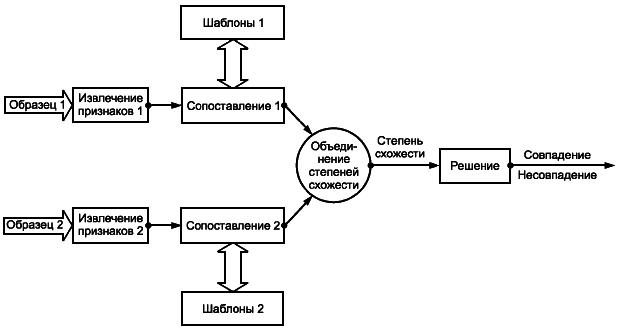
\includegraphics[scale=0.60]{res/bio_b}
\caption{объединение на уровне степеней схожести}
\end{figure}

\item уровень признаков: каждый элементарный биометрический процесс предоставляет на выходе набор признаков, которые объединяются в один набор признаков или вектор;

\begin{figure}[h!]
\centering
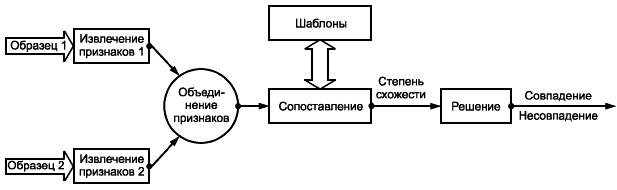
\includegraphics[scale=0.60]{res/bio_c}
\caption{объединение на уровне признаков}
\end{figure}

\item уровень образцов: каждый элементарный биометрический процесс предоставляет на выходе набор образцов, которые объединяются в один образец.

\begin{figure}[h!]
\centering
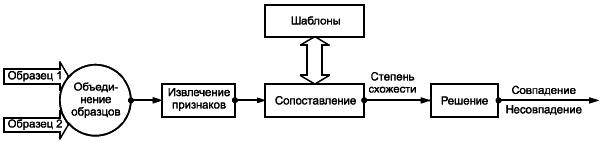
\includegraphics[scale=0.60]{res/bio_d}
\caption{объединение на уровне образцов}
\end{figure}

\end{itemize}

Объединение на первом и втором уровнях происходит до сопоставления, объединение на третьем и четвертом уровнях происходит после сопоставления. Несмотря на то что объединение возможно на всех уровнях, объединение на уровне признаков, на уровне степеней схожести и на уровне принятия решения используют наиболее часто.

%------------------------------------------------

\section{Обзор биометрического распознавания с использованием изображений лица и уха}

Перед тем как рассматривать мультибиометрическое распознавание необходимо рассмотреть обычное биометрическое распознавание, для каждой из частей тела.


%------------------------------------------------

\subsection{Распознавание 2D лица}

Распознавание лиц для человека является регулярной процедурой.
Но вот автоматицзация этого процесса в компьютерном зрении - активное поле для изучения.
Для проверок систем распознавания лица используется The Face Recognition Vendor Test(FRVT).


%------------------------------------------------

\subsection{Метод Главных Компонент - Principal Component Analysis (PCA) }

Одним из наиболее известных и проработанных является метод главных компонент (Principal Component Analysis, PCA), основанный на преобразовании Кархунена — Лоэва. 

Первоначально метод главных компонент начал применяться в статистике для снижения пространства признаков без существенной потери информации. 
В задаче распознавания лиц его применяют главным образом для представления изображения лица вектором малой размерности (главных компонент), который сравнивается затем с эталонными векторами, заложенными в базу данных. 

Главной целью метода главных компонент является значительное уменьшение размерности пространства признаков таким образом, чтобы оно как можно лучше описывало «типичные» образы, принадлежащие множеству лиц. 
Используя этот метод можно выявить различные изменчивости в обучающей выборке изображений лиц и описать эту изменчивость в базисе нескольких ортогональных векторов, которые называются собственными (eigenface). См рисунок 6.

\begin{figure}[h!]
\centering
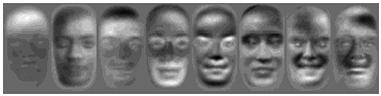
\includegraphics[scale=1.0]{res/pca_faces}
\caption{Пример изображений собственных векторов (собственные лица)}
\end{figure}

Полученный один раз на обучающей выборке изображений лиц набор собственных векторов используется для кодирования всех остальных изображений лиц, которые представляются взвешенной комбинацией этих собственных векторов. 
Используя ограниченное количество собственных векторов можно получить сжатую аппроксимацию входному изображению лица, которую затем можно хранить в базе данных в виде вектора коэффициентов, служащего одновременно ключом поиска в базе данных лиц. 

Суть метода главных компонент сводится к следующему. 
Вначале весь обучающий набор лиц преобразуется в одну общую матрицу данных, где каждая строка представляет собой один экземпляр изображения лица, разложенного в строку. 
Все лица обучающего набора должны быть приведены к одному размеру и с нормированными гистограммами. 
Пример преобразований обучающего набора лиц в одну общую матрицу X представлен на рисунке 7.

\begin{figure}[h!]
\centering
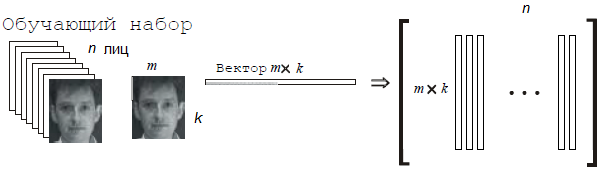
\includegraphics[scale=0.70]{res/ex_set_faces}
\caption{Преобразования обучающего набора лиц в одну общую матрицу X}
\end{figure}

Затем производится нормировка данных и приведение строк к 0-му среднему и 1-й дисперсии, вычисляется матрица ковариации. 
Для полученной матрицы ковариации решается задача определения собственных значений и соответствующих им собственных векторов (собственные лица).
Далее производится сортировка собственных векторов в порядке убывания собственных значений и оставляют только первые k векторов по правилу представленному на рисунке 8.

\begin{figure}[h!]
\centering
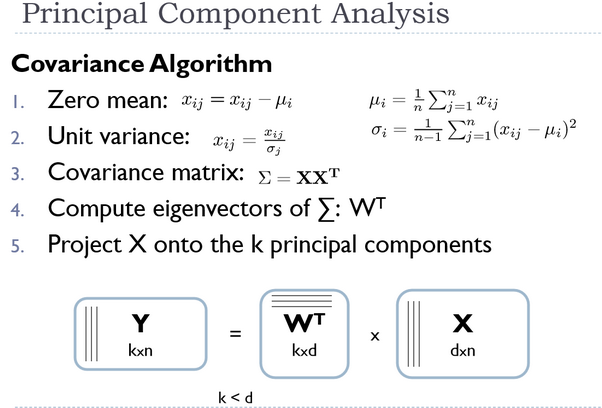
\includegraphics[scale=0.70]{res/pca_rules}
\caption{Алгоритм РСА}
\end{figure}

Принцип выбора базиса из первых лучших собственных векторов представлен на рисунке 9.

\begin{figure}[h!]
\centering
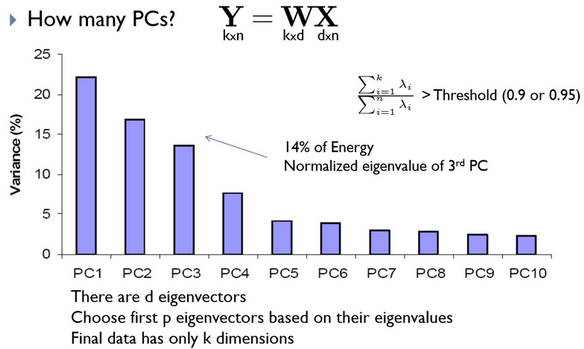
\includegraphics[scale=0.70]{res/pick_bases}
\caption{Принцип выбора базиса из первых лучших собственных векторов}
\end{figure}

На рисунке 10 можно увидеть пример отображения лица в трехмерное метрическое пространство, полученном по трем собственным лицам и дальнейшее распознавание.

\begin{figure}[h!]
\centering
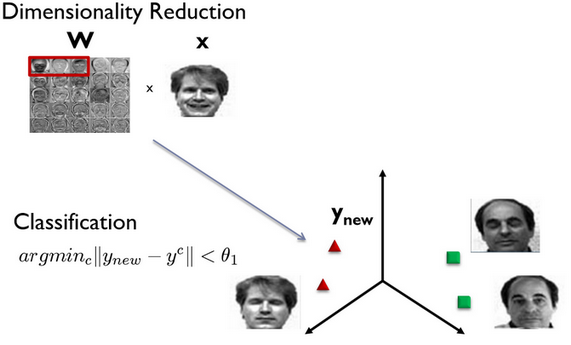
\includegraphics[scale=0.70]{res/pick_bases_ex}
\caption{Отображение лица в трехмерное метрическое пространство}
\end{figure}

Метод главных компонент хорошо зарекомендовал себя в практических приложениях.
Преимущества метода:

\begin{itemize}
\item при наличии в наборе изображений лиц вариаций, таких как раса, пол, эмоции, освещение, будут появляться компоненты, величина которых в основном определяется этими факторами. Поэтому по значениям соответствующих главных компонент можно определить, например, расу или пол человека
\item хранение и поиск изображений в больших базах данных, реконструкция изображений
\end{itemize}
Основная трудность состоит в высоких требованиях к условиям съёмки изображений. 
Изображения должны быть получены в близких условиях освещённости, одинаковом ракурсе (решается добавлением в обучающую выборку изображений в различных ракурсах) и должна быть проведена качественная предварительная обработка, приводящая изображения к стандартным условиям.
В тех случаях, когда на изображении лица присутствуют значительные изменения в освещенности или выражении лица, эффективность метода значительно падает. 
Все дело в том, что PCA выбирает подпространство с такой целью, чтобы максимально аппроксимировать входной набор данных, а не выполнить дискриминацию между классами лиц. 



%------------------------------------------------

\subsection{2D распознавание уха}

Первым, кто разработал систему распознавания ушей - Янарелли. 
Изображение доводили до стандартной позиции, а измерения функции уха производились вручную.
Эта система использует двенадцать частей уха, а также расовую и гендерную информацию, чтобы однозначно идентифицировать объекты(см. рисунок 11).

\begin{figure}[h!]
\centering
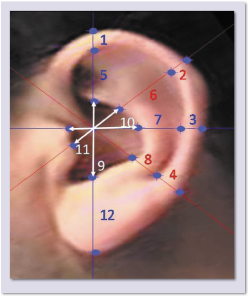
\includegraphics[scale=0.70]{res/twelve_parts}
\caption{В системе идентификации Янарелли используются 12 геометрических измерений, центральным элементом которых является ножка завитка}
\end{figure}

После Пун и Мун сделали обзор биометрии уха.
Они сделали вывод, что меньший размер уха и однородные цвета - содействуют более точному распознаванию.
А основные методы для распознавания ушей - PCA, преобразование силового поля(force field transformation), диаграммы Вороного, нейронные сети и генетические алгоритмы.

Производительность PCA зависит от расположения контрольных точек лица.
Так например, Чанг использует треугольную ямку и межкозелковую вырезку.
А Ян использует, также треугольную ямку и противокозелок.
На рисунке 12 представлены данные точки.

\begin{figure}[h!]
\centering
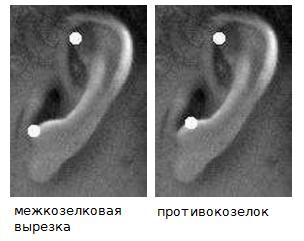
\includegraphics[scale=0.70]{res/diff_ears}
\caption{На левом изображении треугольная ямка и межкозелковая вырезка. На рисунке справа треугольная ямка и противокозелок.}
\end{figure}

Проводился эксперимент зависимости размера. На рисунке 13 представлен график эффекта сдвига при использовании разных размеров.

\begin{figure}[h!]
\centering
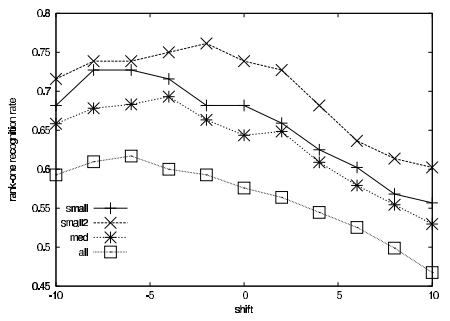
\includegraphics[scale=0.70]{res/shift_eff}
\caption{Эффект сдвига в зависимости от размера}
\end{figure}



%------------------------------------------------

\subsection{3D распознавание лица}

Результаты опроса Бойера показали, что в основном используются две категории распознавания.
Одна из них использует 3D модели для распознавания.
Другая мультибиометрические методы, комбинируя 3D модели и 2D изображения.

На данный момент системы 3D распознавания лиц используют специальное оборудование для реконструкции трехмерной модели лица (сенсорные системы). Сенсорные технологии 3D распознавания делятся на три категории: 

\begin{itemize}
\item Стерео. Используются две камеры с известным взаиморасположением для получения стереопары изображений объекта; на полученных изображениях находятся соответствующие точки и вычисляется положение сопоставленных точек в трехмерном пространстве. 
\item Структурированный свет. Этот подход использует камеру и световой проектор: структурный свет проецирует на лицо специальную текстуру, а камера регистрирует искажения этой текстуры на объемном объекте. С помощью методов восстановления формы по текстуре вычисляется расположение точек в  трехмерном пространстве. 
\item Лазерное сканирование. Лазерные сканеры применяют свет как источник для обнаружения расстояния до объекта сканирования. Они измеряют время отражения лазера от объекта и получают информацию о глубине расположения точек на его поверхности.
\end{itemize}

Системы 3D распознавания лиц, не использующие дополнительное оборудование, существуют только в качестве опытных разработок и коммерческого применения пока не имеют. 

Для того чтобы получить трехмерную информацию об объекте, используются алгоритмы, объединенные в англоязычной литературе под названием «shape from X» (получение формы с помощью Х), где под Х понимаются самые различные методы.

Способы получения трехмерной информации о лице:
\begin{itemize}
\item Восстановление формы по теням (shape from shading, SFS)
\item Восстановление формы по стереопаре (shape from stereo)
\item Восстановление формы по движению (shape from motion, SFM)
\end{itemize}

Среди различных подходов 3D распознавания можно выделить три основных: анализ формы 3D поверхности лица, статистические подходы и использование параметрической модели лица.

\begin{itemize}
\item Анализ формы 3D поверхности. 
Методы, основанные на анализе формы трехмерного изображения лица, используют локальные или глобальные характеристики поверхности, которая описывает лицо, например, кривизну, профили линий, метрики расстояний между двумя поверхностями

\item Статистические методы. 
В частности метод главных компонент, ранее широко использовались в 2D распознавании. 
Метод PCA реализован также для 3D распознавания и был расширен одновременно на комбинацию карт глубины и цвета. Альтернативным для PCA является метод линейного дискриминантного анализа, в котором, в отличие от PCA, один объект (заданный человек) задается не одним лицом, а набором моделей (3D лиц).
Еще одним статистическим методом, также позаимствованным из 2D распознавания, является метод скрытых марковских моделей (СММ). 
Теория Марковских случайных полей позволяет строить оценки различных пространственно-переменных величин по изображениям, при этом накладывая на эти величины определенные априорные ограничения. 
В качестве таких пространственно-переменных величин могут выступать, например, значения смещения в задаче стереореконструкции. 
В литературе по 3D распознаванию этот метод известен как псевдо 3D скрытые марковские модели и используется, в частности, для распознавания выражений лиц. 
\item Использование параметрической модели лица. 
Ключевая идея распознавания по моделям основана на так называемых параметрических 3D моделях, когда форма лица контролируется набором параметров (коэффициентов) модели. 
Эти коэффициенты описывают 3D форму лица и также могут задавать цвет (текстуру) на ее поверхности. 
Данный метод использует на входе одно или несколько изображений лица, в основном фотографий, полученных в анфас и профиль. 
\end{itemize}

Рассмотренные выше способы восстановления трехмерной модели лица имеют ограничения и недостатки, которые не позволяют с их помощью решить задачу распознавания лиц по видеопоследовательности эффективно. 
Методы восстановления формы по движению, основанные на факторизации матриц, восстанавливают трехмерные координаты только некоторых точек объекта, поэтому возникает задача интерполяции его поверхности между восстановленными точками модели. 
Восстановление трехмерной сцены по паре изображений, полученных с разных ракурсов, может дать точный трехмерный образ практически для всех точек исходной сцены, но требует высокой точности данных о взаиморасположении камер. 
Методы получения формы по теням не способны корректно восстанавливать трехмерную информацию об объекте в реальных условиях, когда характер освещения неизвестен и может произвольно изменяться. 


%------------------------------------------------

\subsection{3D распознавание уха}

Для 3D распознавания уха применяют ICP алгоритм.
Итеративный алгоритм ближайших точек (англ. Iterative Closest Point — ICP) — алгоритм, использующийся для сведения к минимуму разницы между двумя облаками точек. 

\begin{figure}[h!]
\centering
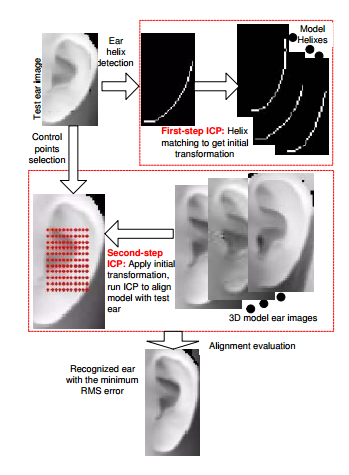
\includegraphics[scale=1.0]{res/icp_steps}
\caption{Диаграмма 3D распознавания уха}
\end{figure}

ICP часто используется для восстановления двухмерных (2D) или трёхмерных (3D) поверхностей из разных изображений.
Алгоритм концептуально прост и часто используется в режиме реального времени.
Чен и Бану выделили три этапа 3D распознавания уха с использованием алгоритма ICP.
\begin{itemize}
\item автоматическое определение спирали уха
\item первый шаг ICP алгоритма для выравнивания спирали модели уха со спиралью тестового уха и получение изометрии
\item второй шаг ICP алгоритма для получения результата трансформации
\end{itemize}

Для каждой модели запускается IPC алгоритм для сравнения ее с тестовыми данными.


\begin{figure}[h!]
\centering
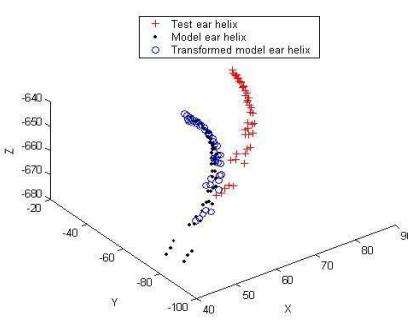
\includegraphics[scale=1.0]{res/icp_step_2}
\caption{Выравнивание спирали модели уха и тестового уха}
\end{figure}

При этом облаком точек является облако точек спирали (См. рисунок 15).
После этого мы имеем набор изометрий для каждой пары модель-тест.
На втором шаге ICP алгоритма для лучшего распознавания сравнение производится по контрольным точкам для каждой пары модель-тест.
Вычисляется среднее квадратичное (root mean square, RMS) зарегистрированных ошибок для каждой такой пары. 
Модель из пары с наименьшим RMS ошибок считается распознанным ухом.

Результат второго шага можно увидеть на рисунке 16.

\begin{figure}[h!]
\centering
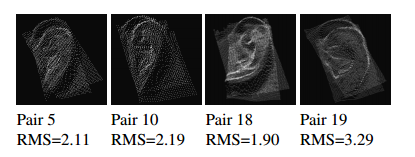
\includegraphics[scale=1.0]{res/icp_step_3}
\caption{Пример определения наименьшего RMS ошибок}
\end{figure}

%------------------------------------------------

\subsection{Совместное применение}

Мультибиометрические системы комбинирующие лицо и ухо изначально были мульти-экземплярными системами.
Для каждой части использовались одинаковые сенсоры, но при этом применялись различные алгоритмы.
Кроме того, несколько датчиков могут быть важны для того, чтобы захватить сразу несколько частей.
Например, система камер установленная вокруг лица может захватить как лицо, так и ухо.
Рассмотрим эксперимент мульти-экземплярной биометрии похожий на те, что проводил Чанг.
Образцы для эксперимента были получены после двухшаговой обработки: нормализация изображения и наложение маски.
Точки ландмарка были проставлены оператором.
Для лица - центры глаз.
Для ушей - треугольная ямка.

Затем, каждая по отдельности, части были обработаны алгоритмом PCA.
Для каждой части было использовано 411 объектов галереи.
Генерировался файл с расстоянием до каждого изображения галереи.
Расстояние ранжировалось косинусом Махаланобиса от -1 до 1, где -1 лучший возможный ранг, 1 соответственно худший.
На рисунке 17 приводится пример таблицы дистанций для объекта 02463.
При этом как метрика дистанции используется косинус Махаланобиса.

\begin{figure}[h!]
\centering
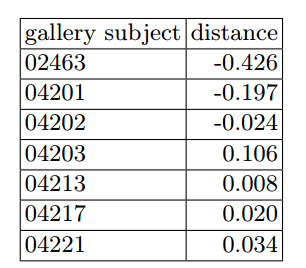
\includegraphics[scale=0.60]{res/distances_table}
\caption{Таблица дистанций}
\end{figure}

\begin{figure}[h!]
\centering
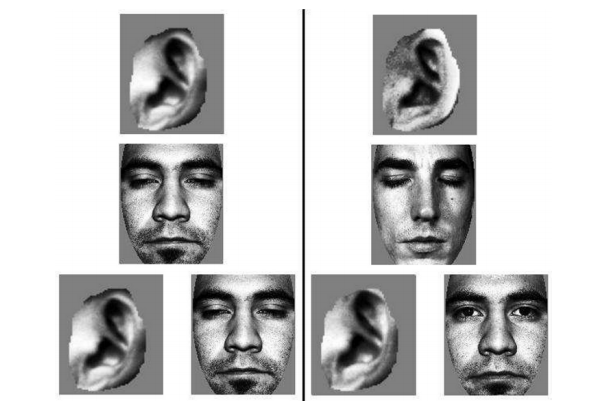
\includegraphics[scale=1.0]{res/ex_individual_failed}
\caption{Пример со слиянием и индивидуальное распознавание. Слева - образцы, справа найденные изображения из галереи }
\end{figure}

После этого производится слияние результатов.
Можно выбрать разные способы слияния.
Например, суммировать расстояния, можно выставлять вес скажем 0.7 для уха и 0.3 для лица или наоборот. 
Так же можно выбирать минимальное значение.
В данном эксперименте результативность распознавания составила 100\%.
В свою очередь индивидуальное сопоставления при использовании PCA удавалось не во всех случаях.
На рисунке 18 можно увидеть пример, в котором по индивидуальным образцам распознавание было не успешным.

\begin{figure}[h!]
\centering
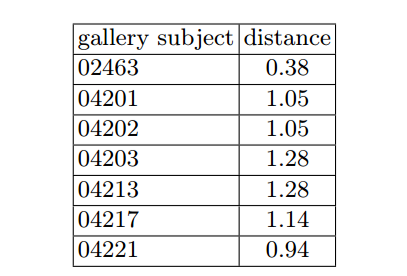
\includegraphics[scale=0.60]{res/distances_table_2}
\caption{Таблица дистанций}
\end{figure}

Следующий пример - мульти-модальный.
Он использует мульти-экземпляр - ухо и лицо, мульти-сенсор - 2D и 3D, мульти-алгоритм - PCA и ICP.
Для данного эксперимента также были использованы 411 объектов галереи.
Для каждой пары вычисляется изометрия используя алгоритм ICP.
RMS расстояния между ближайшими точками сравниваемых изображений заносились в таблицу и использовались как показатель распознавания.
Чем меньше показатель тем ранг распознавания выше.
На рисунке 19 приводится фрагмент таблицы для распознавания образца 02463.
Показатель распознавания для лица с алгоритмом PCA - 88.1\%, уха с алгоритмом ICP - 91.6\%.
Далее производится слияние результатов.
Для ICP результаты могут быть в диапазоне от 0 до бесконечности.
Для PCA от -1 до 1.
Для обоих случаев чем меньше, тем лучше.
Для нормализации результатов используется метод min-max.
Показатель вычисляются по формуле:
$s_i^\prime = \frac{s_i - min_i}{min_i - max_i}$
, где $min_i$ и $max_i$ - соответственно минимальные и максимальные значения из наборов.

\begin{figure}[h!]
\centering
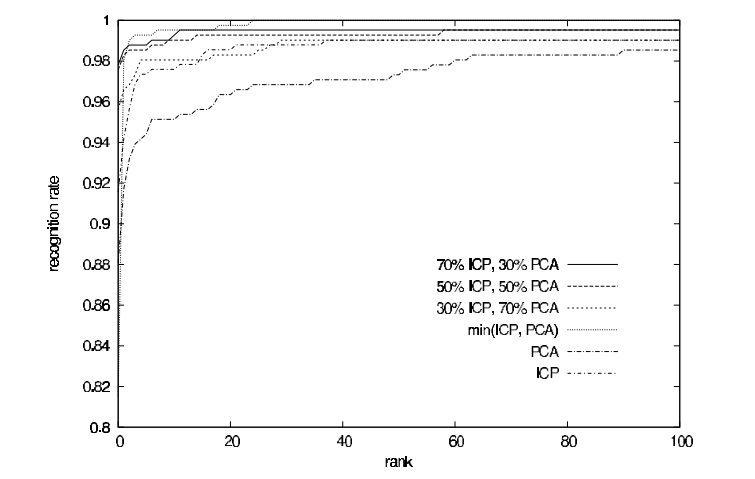
\includegraphics[scale=0.60]{res/fusion_rates}
\caption{Сравнение вариантов слияния}
\end{figure}

Таким образом результирующий показатель будет в диапазоне от 0 до 1.
Так же, как и в предыдущем примере возможны различные варианты слияния. 
Результаты каждого из них приведены на рисунке 20.

%------------------------------------------------

\section{Вывод}

При использовании сочетания образцов лица и уха качество распознавания улучшается по сравнению с результатами индивидуального распознавания.
Так, например, лицо больше, но подвержено изменениям со временем. 
Ухо в свою меньше, но с течением времени изменения гораздо не значительнее по сравнению с лицом.
Преимуществом 2D методов является то, что захват образца производится проще.
"Регулярные" образцы захватываются в доли секунды.
С другой стороны 2D образцы не имеют понятия "глубины".
Преимущество использования и уха и лица в том, что вместе они увеличивают количество биометрических признаков.
В ситуации когда ухо закрыто волосами можно распознать только по лицу.
Тем не менее для такого распознавания требуется больше оборудования.
В случае совмещения 2D и 3D образцов требуется больше сенсоров.
Часто в мультибиометрических системах некоторые этапы предварительной подготовки производятся вручную.
Автоматизация этого процесса затруднена качеством образцов, например, при плохом освещении.
Автоматическая сегментация уха до сих пор является активно исследуемой темой.
Помимо прочего, важна производительность.
В случае использования системы распознавания в целях безопасности от нее не будет толка, если данные в итоге будут получены через длятельное время, например, в течении часа.

%------------------------------------------------

\section{Список литературы}

\addcontentsline{toc}{section}{Список используемой литературы}

Ссылки:

\begin{enumerate}

\item Anil K. Jain Handbook of Biometrics. / Patrick Flynn, Arun A. Ross. - NY: Springer Science+Business Media, LLC, 2008. - 556 c

\item blackcat87 Анализ существующих подходов к распознаванию лиц. - / Электронные данные. - Блог компании Синезис - \\ http://habrahabr.ru/company/synesis/blog/238129/

\item Hui Chen and Bir Bhanu. Contour Matching for 3D Ear Recognition. / - Center for Research in Intelligent Systems, University of California, Riverside, California 92521, USA

\item Ping Yan and Kevin W. Bowyer. Empirical Evaluation of Ear Biometrics. / - Department of Computer Science and Engineering
University of Notre Dame, IN 46556

\item tibult Исследование метода главных компонент и линейного дискриминантного анализа на изменение ракурса и условий освещенности лица как объект распознавания. / Электронные данные. - http://habrahabr.ru/post/197974/

\item Визильтер, Ю.В. Обработка и анализ изображений в задачах машинного зрения: Курс лекций и практических занятий. / Желтов С.Ю., Бондаренко А.В., Ососков М.В., Моржин А.В. – М.: Физматкнига, 2010. – 672 с.

\item ГОСТ Р 54411-2011/ISO/IEC/TR 24722:2007 Информационные технологии. Биометрия. Мультимодальные и другие мультибиометрические технологии. - М.: Стандартинформ, 2014

\item Дьяченко А.В. Задача 3D распознавания лиц: современные методы решения. / Институт проблем искусственного интеллекта МОН Украины и НАН Украины, Донецк

\item Каркищенко А. Н. Гречухин И. А. СТАТИСТИЧЕСКОЕ РАСПОЗНАВАНИЕ ЛИЦ ПО ГЕОМЕТРИИ ХАРАКТЕРНЫХ ТОЧЕК ДЛЯ СИСТЕМ ТРАНСПОРТНОЙ БЕЗОПАСНОСТИ. / Журнал, Управление большими системами: сборник трудов Выпуск № 38 / 2012.

\item Мокеев А. В. О ТОЧНОСТИ И БЫСТРОДЕЙСТВИИ МЕТОДА СИНТЕЗА ГЛАВНЫХ КОМПОНЕНТ. / Журнал, Бизнес-информатика Выпуск № 3 / 2010.

\end{enumerate}

\end{document}